\documentclass[11pt]{article}

\usepackage{graphicx}

\title{Practicing with an offline dictionary attack \\\large HW2 - CNS Sapienza}
\author{Matteo Salvino 1708108}
\date{14 November 2019}

\begin{document}
\maketitle

\section{Goal}
In this CNS homework we are interested to do some practice on cryptography field, in particular regarding offline dictionary attack. The main goal is to decrypt a given ciphertext, obtained executing the following command : 
\begin{center}
openssl enc -aes-192-cbc -pbkdf2 -e -in <infile.txt> -out ciphertext.enc
\end{center}
An important note is that it was used OpenSSL version 1.1, and to make things work we will do the same. In the next section, we will analyze what we know about ciphertext, plaintext and the key used.
\section{Knowledge exploiting}
Let's start analyzing the previous command. To encrypt our plaintext target file, it was used \textit{AES} with 192 bits key length as symmetric encryption algorithm. A thing to notice is that it was used the flag \textit{pbkdf2}. This flag allow us to use key derivation function version 2 in order to generate several secret keys from a given passphrase or password. In order to find the corresponding plaintext we need to use the same algorithm with this flag, but in decryption mode, and give a passphrase that will be manipulated from the derivation function. Passing to the passphrase we know that is an english meaningful word. Finally, we know that the plaintext is english text.
\section{Dictionary selection}
Exploring the web we found an interesting english words dictionary. It contains a list of the 10k most common english words in order of frequency (descending order). It was built from other bigger dictionaries and does not contains spaces, numbers and bad words. In particular, it contains three type of word :
\begin{itemize}
\item \textbf{Short} : Word's length between 1 and 4 characters.
\item \textbf{Medium} : Word's length between 5 and 8 characters.
\item \textbf{Long} : Word's length greater or equal than 9 characters.
\end{itemize}
Furthermore, this dictionary contains also american spelling words. We know that the passphrase is english word, yes but we feel safer including also this last spelling.
\section{Attack prototype}
First of all, we will launch the offline dictionary attack on a linux machine version 18.04. We think that the fastest way to prepare this type of attack is to write a bash script in order to try different passphrases, and see if it was right or not. In particular, we store in a variable called input the path to the dictionary we will use, then we will read the dictionary line by line, launching the following command :
\begin{center}
 openssl enc -aes-192-cbc -pbkdf2 -d -in ./ciphertext.enc -out ./plaintext.txt -pass pass:\$line
\end{center}
where \$line represent the current passphrase. Notice that we will use the flag pass in order to provide the current passphrase to the decryption algorithm, simplifying the script's life. The return value of this command is zero in case of success, otherwise a specific value in case of failure. Furthermore, we know that if we provide a wrong passphrase OpenSSL will give back a decryption error (i.e. return value different from zero). So, if the return value is zero, the current passphrase can be right. Why can it be right, and not definitely right ? Because we could find a passphrase that decrypt the given ciphertext, but the corresponding plaintext's type is not the ascii one, having a meaningless text. Passphrases of this type are called \textbf{false positive}. Then, to avoid this cases, a further check is required. In particular, we will need to check if the plaintext produced at each iteration, have the ascii format or not. In the positive case, we have completed the offline attack (stopping the loop), because we found a meaningful english text decrypting the given ciphertext. In the negative case, we found a false positive, then we proceed with next line of the dictionary. In the worst case, if the chosen dictionary is not big enough then we will not find the right passphrase. Fortunately, we aren't in the worst case, because we got the right passphrase (i.e. "learning") with the corresponding plaintext, as you can see in the following picture 
\begin{center}
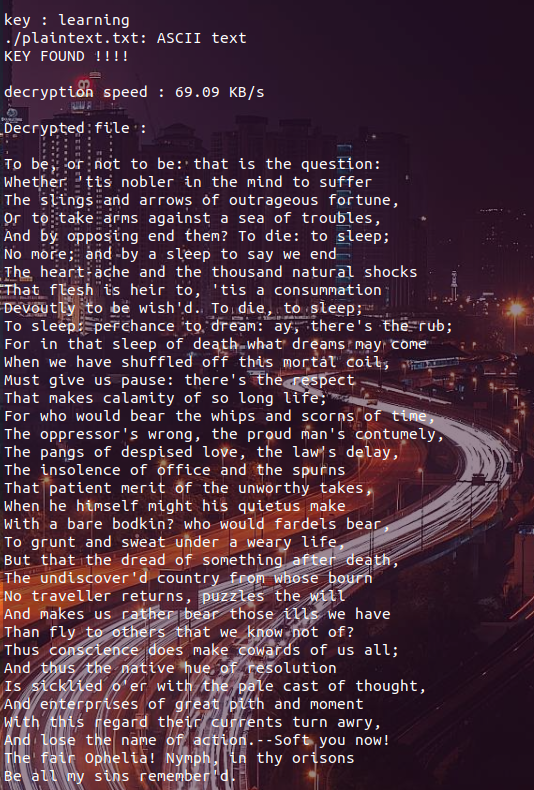
\includegraphics[scale=0.4]{./successfully_attack.png}
\end{center}
We measured the decryption speed via a system's function called date, and we got a speed around $69.09$ KB/s.
\section{Conclusions}
We could seen that with a certain knowledge level of the encryption domain, it is not impossible to conclude successfully an offline dictionary attack. Naturally, in our case we know all possible informations except the plaintext. There can be some cases in which we know nothing at all, thus the search of right key can take a lot of time. With this homework we learned how we should work in situations in which is possible to take the role of the attackers.
\end{document}